% !TEX program = xelatex
% c5p-s-2026.tex
% 2026 €€£ 非专业级别软件能力认证第一轮（C5P-S1）提高级 C++语言试题（模拟卷）
% 版式：a4paper、等线题头、宋体中文 + Consolas 西文、页脚两行（PDF 格式）、选项每行一个、大题强制换页
% 代码：带边框、左侧行号 0 补齐、无横向线条；阅读程序不写概要，完善程序写概要后挖空
% 编译方式：xelatex c5p-s-2026.tex（建议编译两次）
\documentclass[a4paper]{ctexart}

\usepackage{fontspec}
\usepackage{graphicx}
\usepackage{tikz}
\usetikzlibrary{arrows.meta}
\usepackage{eso-pic}
\newcommand{\waterword}{%
  \makebox[0pt][c]{%
    \tikz[baseline]{%
      \node[
        inner sep=0pt,
        rotate=-35,
        text=black,
        opacity=0.085,
        font=\fontsize{54}{70}\selectfont
      ] {折工};%
    }%
  }%
}
\AddToShipoutPictureFG{%
  \put(\LenToUnit{-0.3cm},\LenToUnit{1.2cm}){\waterword}%
  \put(\LenToUnit{5.0cm},\LenToUnit{0.0cm}){\waterword}%
  \put(\LenToUnit{10.3cm},\LenToUnit{1.4cm}){\waterword}%
  \put(\LenToUnit{15.6cm},\LenToUnit{0.2cm}){\waterword}%
  \put(\LenToUnit{2.2cm},\LenToUnit{6.2cm}){\waterword}%
  \put(\LenToUnit{7.5cm},\LenToUnit{4.8cm}){\waterword}%
  \put(\LenToUnit{12.8cm},\LenToUnit{6.3cm}){\waterword}%
  \put(\LenToUnit{18.1cm},\LenToUnit{4.9cm}){\waterword}%
  \put(\LenToUnit{-0.3cm},\LenToUnit{10.0cm}){\waterword}%
  \put(\LenToUnit{5.0cm},\LenToUnit{11.5cm}){\waterword}%
  \put(\LenToUnit{10.3cm},\LenToUnit{10.1cm}){\waterword}%
  \put(\LenToUnit{15.6cm},\LenToUnit{11.6cm}){\waterword}%
  \put(\LenToUnit{2.2cm},\LenToUnit{16.5cm}){\waterword}%
  \put(\LenToUnit{7.5cm},\LenToUnit{15.1cm}){\waterword}%
  \put(\LenToUnit{12.8cm},\LenToUnit{16.6cm}){\waterword}%
  \put(\LenToUnit{18.1cm},\LenToUnit{15.2cm}){\waterword}%
  \put(\LenToUnit{-0.3cm},\LenToUnit{21.6cm}){\waterword}%
  \put(\LenToUnit{5.0cm},\LenToUnit{23.1cm}){\waterword}%
  \put(\LenToUnit{10.3cm},\LenToUnit{21.7cm}){\waterword}%
  \put(\LenToUnit{15.6cm},\LenToUnit{23.2cm}){\waterword}%
  \put(\LenToUnit{2.2cm},\LenToUnit{27.3cm}){\waterword}%
  \put(\LenToUnit{7.5cm},\LenToUnit{25.9cm}){\waterword}%
  \put(\LenToUnit{12.8cm},\LenToUnit{27.4cm}){\waterword}%
  \put(\LenToUnit{18.1cm},\LenToUnit{26.0cm}){\waterword}%
}
\usepackage{geometry}
\geometry{top=2.7cm, left=2.7cm, right=2.7cm, bottom=4cm}
\setmainfont{Consolas}
\setmonofont{Consolas}
\setCJKmainfont{SimSun}
\newCJKfontfamily{\dengxian}{DengXian}

\usepackage{fancyhdr}
\usepackage{lastpage}
\usepackage[most]{tcolorbox}
\usepackage{listings}
\usepackage{enumitem}
\usepackage{amsmath}
\usepackage{xcolor}
\DeclareMathSizes{10.53937}{10.95}{7.5}{5.5}

% 将带圈数字 ①-⑤ 划入 CJK 字符类，确保题干“①处应填”用中文字体正常渲染
\xeCJKDeclareCharClass{CJK}{"2460 -> "2464}

% ---------------- 页脚：中文宋体 + 数字英文 Times New Roman（参考 cspjs2024hs.pdf 样式） ----------------
\newfontfamily\trm{Times New Roman}
% 普通 Unicode 黑圆点，避免依赖 Wingdings 私有字形映射
\newcommand{\wdot}{{\fontsize{12}{12}\selectfont\textbullet}}
\pagestyle{fancy}
\fancyhf{}
\setlength{\footskip}{1.5cm}
\fancyfoot[C]{{\xeCJKsetup{CJKecglue={\hskip0pt}}{\trm €€£ C5P-S 2026 }{\songti 第一轮 }{\trm C++}{\songti 语言试题}}\\[2pt]{\xeCJKsetup{CJKecglue={\hskip0pt}}{\songti 第}{\trm\thepage}{\songti 页，共}{\trm\pageref{LastPage}}{\songti 页}}}
\renewcommand{\headrulewidth}{0pt}
\renewcommand{\footrulewidth}{0pt}

% ---------------- 代码样式：框宽 14cm、Consolas 12pt、行号 8.5pt(约0.3cm高)、关键字不加粗 ----------------
\renewcommand{\thelstnumber}{\ifnum\value{lstnumber}<10 0\fi\arabic{lstnumber}}
\lstset{
  language=C++,
  basicstyle=\ttfamily\fontsize{12}{14.4}\selectfont,
  numberstyle=\ttfamily\fontsize{12}{14.4}\selectfont\makebox[0.92cm][r],
  numbers=left,
  numbersep=0.08cm,
  frame=none,
  framesep=6pt,
  rulecolor=\color{black!70},
  columns=fullflexible,
  keepspaces=true,
  aboveskip=0pt,
  belowskip=0pt,
  xleftmargin=0.88cm,
  linewidth=13cm,
  showstringspaces=false,
  breaklines=true,
  breakatwhitespace=false,
  keywordstyle=\ttfamily,
  commentstyle=\ttfamily,
  stringstyle=\ttfamily,
  escapeinside={|@}{@|},
}

% 代码框：线1（左框线）距页左 2.05cm；行号列线1→线2 严格 1cm；代码列线2→线3 严格 13cm；
% 线3（右框线）距页右约 4.95cm（A4 宽 21cm 自动吻合）；挖空下划线 2.10cm + 居中序号
\newtcolorbox{codebox}{enhanced, breakable, sharp corners, boxrule=0.5pt, colframe=black, colback=white,
  width=13.45cm, left skip=-0.65cm, before skip=6pt, after skip=8pt,
  top=2pt, bottom=2pt, left=0pt, right=0pt,
  overlay={\draw[black,line width=0.5pt] ([xshift=1.0cm]frame.north west)--([xshift=1.0cm]frame.south west);}}
% 完善程序挖空：2.10cm 下划线 + 居中序号（字体同代码 12pt）
\newcommand{\blank}[1]{\underline{\makebox[2.1cm][c]{#1}}}

\setlength{\parindent}{0pt}
\setlength{\parskip}{2pt}
\linespread{1.25}

% 大题标题（左对齐黑体）
\newcommand{\bigtitle}[1]{\noindent\heiti #1\par\vspace{2pt}}
% 小题题干（序号数字不加粗，Consolas）
\newcommand{\q}[1]{\noindent #1}
% 阅读程序小题：题号前加 Unicode 黑点（整体左对齐）
\newcommand{\qdot}[1]{\noindent\wdot\hspace{0.6em}#1}
% 单个选项（每个选项独立一行）
\newcommand{\opt}[1]{\hspace*{2em} #1\par}
% 完善程序选项：两个选项一行（A B 一行、C D 一行）
\newcommand{\optw}[2]{\hspace*{2em} #1\hspace*{2em}#2\par}

\begin{document}

\begin{center}
{\dengxian
    {\xeCJKsetup{CJKecglue={\hskip 0.419em}}\fontsize{15.95}{1}\selectfont 2026 €€£非专业级别软件能力认证第一轮} \\[1.5em]
    {\xeCJKsetup{CJKecglue={\hskip 0.419em}}\fontsize{15.95}{1}\selectfont （C5P-S1） 提高级 C++\hspace{0pt}语言试题} \\[1.5em]
    {\xeCJKsetup{CJKecglue={\hskip 0.344em}}\fontsize{14.05}{1}\selectfont 认证时间：2026年9月26日14:30\textasciitilde16:30}
}
\end{center}

\vspace{8pt}
\noindent{\heiti 考生注意事项：}
\begin{itemize}[leftmargin=2.6em, itemsep=1pt, label={}]
    \item \wdot\hspace{0.5em}试题纸共有 \pageref{LastPage} 页，答题纸共有 1 页，满分 100 分。本卷为自制模拟卷，不代表任何官方机构。
    \item \wdot\hspace{0.5em}本卷按《全国青少年信息学奥林匹克系列竞赛大纲（2025 年修订版）》提高级及其自动包含的入门级知识范围命制。
    \item \wdot\hspace{0.5em}不得使用任何电子设备（如计算器、手机、电子词典等）或查阅任何书籍资料。
\end{itemize}

\bigtitle{一、单项选择题（共 15 题，每题 2 分，共计 30 分；每题有且仅有一个正确选项）}
\q{1.} 在 Linux 终端中，将源文件 \texttt{main.cpp} 编译为名为 \texttt{main} 的可执行文件，应使用的命令是（\qquad）\\
\opt{A. \texttt{g++ main.cpp -o main}}\opt{B. \texttt{g++ main -o main.cpp}}
\opt{C. \texttt{./main.cpp -o main}}\opt{D. \texttt{g++ -o main.cpp main}}

\q{2.} 一棵哈夫曼树用二叉链表存储，共有 254 个非空孩子指针。该树有（\qquad）个叶子结点\\
\opt{A. 127}\opt{B. 128}\opt{C. 129}\opt{D. 255}

\q{3.} 已知 \(T(1)=\Theta(1)\)，且当 \(n>1\) 时
\[
T(n)=2T(n/2)+\Theta(n\log n),
\]
其中 \(n\) 为 2 的幂。由主定理，\(T(n)\) 为（\qquad）\\
\opt{A. \(\Theta(n\log n)\)}\opt{B. \(\Theta(n\log^2 n)\)}\opt{C. \(\Theta(n^2)\)}\opt{D. \(\Theta(\log^2 n)\)}

\q{4.} 从 \texttt{(0,0)} 出发，每步向右或向上，到达 \texttt{(8,6)}。要求途中始终满足 \texttt{x >= y}，且不经过 \texttt{(4,2)}。这样的路径共有（\qquad）条\\
\opt{A. 443}\opt{B. 558}\opt{C. 630}\opt{D. 1001}

\q{5.} 用两个栈 A、B 模拟队列。入队时压入 A；出队时，若 B 为空，则先把 A 中的元素全部移入 B。初始两栈均为空，依次执行\\
\texttt{push(1), push(2), pop(), push(3), push(4),}\\
\texttt{pop(), push(5), pop(), pop()}。\\
元素从 A 移入 B 的次数为（\qquad）\\
\opt{A. 4}\opt{B. 5}\opt{C. 6}\opt{D. 7}

\q{6.} 将整数 \texttt{1,2,...,12} 依次排在一个圆环上。从中选 4 个数，且任意两个被选的数都不相邻，共有（\qquad）种选法\\
\opt{A. 84}\opt{B. 96}\opt{C. 105}\opt{D. 126}

\q{7.} 执行下列 C++ 代码后，输出为（\qquad）\\
\begin{codebox}\begin{lstlisting}
map<int, int> mp;
mp[2] = 1;
mp[1] = mp[2] + 2;
int x = mp[3];
mp[2] += mp[1];
cout << mp.size() << ' ' << mp[1] + mp[2] + mp[3];
\end{lstlisting}\end{codebox}
\opt{A. \texttt{2 4}}\opt{B. \texttt{2 7}}\opt{C. \texttt{3 4}}\opt{D. \texttt{3 7}}

\q{8.} 用 Kahn 算法对一个有向无环图进行拓扑排序。该图的拓扑序唯一，当且仅当（\qquad）\\
\opt{A. 每个结点的出度都不超过 1}
\opt{B. 算法的每一步中，当前入度为 0 且尚未删除的结点恰好有 1 个}
\opt{C. 图中恰好有 \texttt{n-1} 条边}
\opt{D. 从任意结点开始 DFS 得到的完成时间序列都相同}

\q{9.} 模式串 \texttt{ababaabab} 的 KMP 前缀函数最后一项为（\qquad）\\
\opt{A. 2}\opt{B. 3}\opt{C. 4}\opt{D. 5}

\q{10.} 用邻接矩阵实现朴素 Dijkstra 算法，求一个 \texttt{n} 个顶点的非负权图的单源最短路，其最坏时间复杂度为（\qquad）\\
\opt{A. \texttt{Theta(n)}}\opt{B. \texttt{Theta(m log n)}}\opt{C. \texttt{Theta(n\^{}2)}}\opt{D. \texttt{Theta(nm)}}

\q{11.} 已知 \texttt{p=20260913} 为质数，则
\[
\sum_{i=1}^{p-2}\frac{1}{i(i+1)}\pmod p
\]
的值为（\qquad）\\
\opt{A. 0}\opt{B. 1}\opt{C. 2}\opt{D. \texttt{p-2}}

\q{12.} 在 \texttt{1,2,...,1000} 中，恰好能被 \texttt{2,3,5} 中一个数整除的整数有（\qquad）个\\
\opt{A. 434}\opt{B. 468}\opt{C. 500}\opt{D. 534}

\q{13.} 对下图恰好删去两条不同的边，使得仍存在从 1 到 8 的有向路径。删边方案共有（\qquad）种\\
\begin{center}
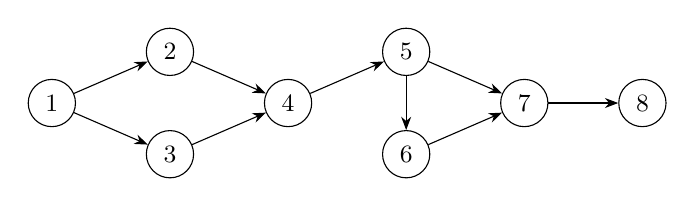
\begin{tikzpicture}[>=Stealth, every node/.style={circle, draw, fill=white, minimum size=6mm, inner sep=0.5pt, font=\small}]
  \node (n1) at (0,0) {1}; \node (n2) at (1.5,0.65) {2}; \node (n3) at (1.5,-0.65) {3};
  \node (n4) at (3,0) {4}; \node (n5) at (4.5,0.65) {5}; \node (n6) at (4.5,-0.65) {6};
  \node (n7) at (6,0) {7}; \node (n8) at (7.5,0) {8};
  \draw[->] (n1)--(n2); \draw[->] (n1)--(n3); \draw[->] (n2)--(n4); \draw[->] (n3)--(n4);
  \draw[->] (n4)--(n5); \draw[->] (n5)--(n6); \draw[->] (n5)--(n7); \draw[->] (n6)--(n7); \draw[->] (n7)--(n8);
\end{tikzpicture}
\end{center}
\opt{A. 12}\opt{B. 15}\opt{C. 18}\opt{D. 21}

\q{14.} 已知整数 \texttt{x} 满足
\[
x\equiv 2\pmod 7,\qquad x\equiv 3\pmod 8,\qquad x\equiv 4\pmod 9.
\]
且 \texttt{0 <= x < 504}，则 \texttt{x}=（\qquad）\\
\opt{A. 247}\opt{B. 355}\opt{C. 499}\opt{D. 503}

\q{15.} 对任意连通无向带权图，下列说法一定正确的是（\qquad）\\
\opt{A. 图中权值最小的每一条边都属于所有最小生成树}
\opt{B. 若一条边是某个环上权值严格最大的边，则它不属于任何最小生成树}
\opt{C. 若一条边属于某一棵最小生成树，则它属于所有最小生成树}
\opt{D. 任意两棵最小生成树包含的边集合一定完全相同}

\clearpage
\bigtitle{二、阅读程序（判断题正确填√，错误填×；判断题每题 1.5 分，普通单选题每题 3 分，第 33 题 4 分，共计 40 分）}

\begin{codebox}\begin{lstlisting}
#include <bits/stdc++.h>
using namespace std;
const int N = 2e5 + 5;
int n, a[N], tmp[N];
long long ans;
void merge_sort(int l, int r) {
    if (l >= r)
        return;
    int mid = (l + r) >> 1;
    merge_sort(l, mid);
    merge_sort(mid + 1, r);
    int i = l, j = mid + 1, k = l;
    while (i <= mid && j <= r) {
        if (a[i] <= a[j])
            tmp[k++] = a[i++];
        else {
            tmp[k++] = a[j++];
            ans += mid - i + 1;
        }
    }
    while (i <= mid)
        tmp[k++] = a[i++];
    while (j <= r)
        tmp[k++] = a[j++];
    for (int p = l; p <= r; ++p)
        a[p] = tmp[p];
}
int main() {
    ios::sync_with_stdio(0);
    cin.tie(0);
    cin >> n;
    for (int i = 1; i <= n; ++i)
        cin >> a[i];
    merge_sort(1, n);
    cout << ans;
}
\end{lstlisting}\end{codebox}

\noindent\wdot\hspace{0.5em}判断题\\
\q{16.} 程序执行结束后，\texttt{ans} 等于原数组的逆序对数。（\qquad）\\
\opt{A. 正确}\opt{B. 错误}
\q{17.} 若 \texttt{i<j} 且 \texttt{a[i]=a[j]}，则这一对元素会使 \texttt{ans} 增加 1。（\qquad）\\
\opt{A. 正确}\opt{B. 错误}
\q{18.} 若把 \texttt{ans} 改为 32 位有符号 \texttt{int}，当 \texttt{n=2e5} 时可能发生溢出。（\qquad）\\
\opt{A. 正确}\opt{B. 错误}

\noindent\wdot\hspace{0.5em}单选题\\
\q{19.} 初始数组为 \texttt{[4,1,3,2,5]}，只调用 \texttt{merge\_sort(1,4)}。调用结束后 \texttt{a[1..5]} 为（\qquad）\\
\opt{A. \texttt{[1,2,3,4,5]}}\opt{B. \texttt{[1,2,4,3,5]}}
\opt{C. \texttt{[1,3,2,4,5]}}\opt{D. \texttt{[4,1,3,2,5]}}
\q{20.} 输入数组为 \texttt{[3,1,2,2,1,3]} 时，程序输出为（\qquad）\\
\opt{A. 5}\opt{B. 6}\opt{C. 7}\opt{D. 8}
\q{21.} 当 \texttt{n=8}，且每次合并的比较次数均达到最大值时，语句 \texttt{a[i] <= a[j]} 共执行（\qquad）次\\
\opt{A. 12}\opt{B. 14}\opt{C. 17}\opt{D. 24}

\begin{codebox}\begin{lstlisting}
#include <bits/stdc++.h>
using namespace std;
int main() {
    ios::sync_with_stdio(0);
    cin.tie(0);
    int n, k;
    string s;
    cin >> n >> k >> s;
    vector<char> st;
    st.reserve(n);
    for (char ch : s) {
        while (k > 0 && !st.empty() && st.back() > ch) {
            st.pop_back();
            --k;
        }
        st.push_back(ch);
    }
    while (k > 0) {
        st.pop_back();
        --k;
    }
    for (char ch : st)
        cout << ch;
}
\end{lstlisting}\end{codebox}

\noindent\wdot\hspace{0.5em}判断题\\
\q{22.} 若 \texttt{k} 的初值为 0，程序不会执行 \texttt{pop\_back()}。（\qquad）\\
\opt{A. 正确}\opt{B. 错误}
\q{23.} 扫描结束后若仍有 \texttt{k>0}，从当前序列末尾继续删除字符是最优的。（\qquad）\\
\opt{A. 正确}\opt{B. 错误}
\q{24.} 该程序的时间复杂度为 \texttt{O(n)}。（\qquad）\\
\opt{A. 正确}\opt{B. 错误}

\noindent\wdot\hspace{0.5em}单选题\\
\q{25.} 输入 \texttt{9 4 cbacdcbca}，扫描完前 6 个字符后，\texttt{st} 从底到顶的内容和 \texttt{k} 的值分别为（\qquad）\\
\opt{A. \texttt{acd, 2}}\opt{B. \texttt{acc, 1}}\opt{C. \texttt{acb, 0}}\opt{D. \texttt{abc, 1}}
\q{26.} 输入 \texttt{8 3 dcabccba} 时，扫描过程中 \texttt{st} 的最大长度为（\qquad）\\
\opt{A. 3}\opt{B. 4}\opt{C. 5}\opt{D. 6}
\q{27.} 输入 \texttt{8 3 dcabccba} 时，程序输出为（\qquad）\\
\opt{A. \texttt{abcba}}\opt{B. \texttt{abccb}}\opt{C. \texttt{acbba}}\opt{D. \texttt{bccba}}

\begin{codebox}\begin{lstlisting}
#include <bits/stdc++.h>
using namespace std;
const int N = 2e5 + 5;
int n, head[N], to[N * 2], nxt[N * 2], ec;
int dista[N], que[N];
void add(int u, int v) {
    to[++ec] = v;
    nxt[ec] = head[u];
    head[u] = ec;
}
int bfs(int start) {
    fill(dista + 1, dista + n + 1, -1);
    int l = 0, r = 0, far = start;
    que[r++] = start;
    dista[start] = 0;
    while (l < r) {
        int u = que[l++];
        if (dista[u] > dista[far])
            far = u;
        for (int e = head[u]; e; e = nxt[e]) {
            int v = to[e];
            if (dista[v] == -1) {
                dista[v] = dista[u] + 1;
                que[r++] = v;
            }
        }
    }
    return far;
}
int main() {
    ios::sync_with_stdio(0);
    cin.tie(0);
    cin >> n;
    for (int i = 1, u, v; i < n; ++i) {
        cin >> u >> v;
        add(u, v);
        add(v, u);
    }
    int s = bfs(1);
    int t = bfs(s);
    cout << dista[t];
}
\end{lstlisting}\end{codebox}

\noindent\wdot\hspace{0.5em}判断题\\
\q{28.} 若有多个最远点，\texttt{bfs} 返回其中最先出队的结点。（\qquad）\\
\opt{A. 正确}\opt{B. 错误}
\q{29.} 对同一棵树，仅改变边的输入顺序，\texttt{bfs(1)} 的返回值可能改变。（\qquad）\\
\opt{A. 正确}\opt{B. 错误}
\q{30.} 对一棵树按程序中的方法进行两次 BFS，最终得到的 \texttt{dista[t]} 等于树的直径。（\qquad）\\
\opt{A. 正确}\opt{B. 错误}
\q{31.} 若输入改为任意连通无权图，两次 BFS 仍一定能求出图的直径。（\qquad）\\
\opt{A. 正确}\opt{B. 错误}

\noindent\wdot\hspace{0.5em}单选题\\
\q{32.} 边按 \texttt{1-2,1-3,2-4,2-5,3-6,3-7} 的顺序输入，\texttt{bfs(1)} 返回（\qquad）\\
\opt{A. 4}\opt{B. 5}\opt{C. 6}\opt{D. 7}
\q{33.}（本题 4 分）树的边为 \texttt{1-2,1-3,2-4,2-5,3-6,3-7} 时，程序输出为（\qquad）\\
\opt{A. 2}\opt{B. 3}\opt{C. 4}\opt{D. 5}

\clearpage
\bigtitle{三、完善程序（单选题，每小题 3 分，共计 30 分）}

\noindent（1）（有序序列的第 K 小和）给定两个长度均为 \texttt{n} 的单调不降序列 \texttt{a}、\texttt{b}。对所有 \texttt{1 <= i,j <= n}，共有 \texttt{n\string^2} 个数 \texttt{a[i]+b[j]}，求其中第 \texttt{k} 小的数。\texttt{1 <= n <= 10\string^5}，\texttt{1 <= k <= n\string^2}，序列元素均为非负整数，答案不超过 \texttt{10\string^9}。
\begin{codebox}\begin{lstlisting}
#include <bits/stdc++.h>
using namespace std;
const int N = 1e5 + 5;
int n, a[N], b[N];
long long k;
long long count_le(long long x) {
    long long cnt = 0;
    int j = |@\blank{①}@|;
    for (int i = 1; i <= n; ++i) {
        while (|@\blank{②}@|)
            --j;
        cnt += |@\blank{③}@|;
    }
    return cnt;
}
long long solve() {
    long long l = |@\blank{④}@|;
    long long r = 1LL * a[n] + b[n];
    while (l + 1 < r) {
        long long mid = (l + r) >> 1;
        if (count_le(mid) >= k)
            r = mid;
        else
            l = mid;
    }
    return |@\blank{⑤}@|;
}
int main() {
    ios::sync_with_stdio(0);
    cin.tie(0);
    cin >> n >> k;
    for (int i = 1; i <= n; ++i)
        cin >> a[i];
    for (int i = 1; i <= n; ++i)
        cin >> b[i];
    cout << solve();
}
\end{lstlisting}\end{codebox}

\q{34.} ①处应填（\qquad）\\
\optw{A. \texttt{n}}{B. \texttt{n-1}}\optw{C. \texttt{1}}{D. \texttt{0}}
\q{35.} ②处应填（\qquad）\\
\opt{A. \texttt{j > 0 \&\& 1LL * a[i] + b[j] > x}}
\opt{B. \texttt{j > 0 \&\& 1LL * a[i] + b[j] >= x}}
\opt{C. \texttt{j < n \&\& 1LL * a[i] + b[j] > x}}
\opt{D. \texttt{j > 0 \&\& 1LL * a[i] + b[j] <= x}}
\q{36.} ③处应填（\qquad）\\
\optw{A. \texttt{j}}{B. \texttt{n-j}}\optw{C. \texttt{j+1}}{D. \texttt{n}}
\q{37.} ④处应填（\qquad）\\
\opt{A. \texttt{1LL * a[1] + b[1]}}
\opt{B. \texttt{0}}
\opt{C. \texttt{1LL * a[1] + b[1] - 1}}
\opt{D. \texttt{1LL * a[n] + b[n]}}
\q{38.} ⑤处应填（\qquad）\\
\optw{A. \texttt{l}}{B. \texttt{r}}\optw{C. \texttt{l+1}}{D. \texttt{count\_le(r)}}

\noindent（2）（最近公共祖先）给定一棵以 1 为根的 \texttt{n} 个结点的树。有 \texttt{q} 次询问，每次给出 \texttt{u,v}，求它们的最近公共祖先。\texttt{1 <= n,q <= 2 * 10\string^5}。
\begin{codebox}\begin{lstlisting}
#include <bits/stdc++.h>
using namespace std;
const int N = 2e5 + 5, K = 19;
int n, q, head[N], to[N * 2], nxt[N * 2], ec;
int dep[N], up[N][K];
void add(int u, int v) {
    to[++ec] = v;
    nxt[ec] = head[u];
    head[u] = ec;
}
void dfs(int u, int p) {
    dep[u] = dep[p] + 1;
    up[u][0] = p;
    for (int j = 1; j < K; ++j)
        up[u][j] = up[|@\blank{①}@|][j - 1];
    for (int e = head[u]; e; e = nxt[e]) {
        int v = to[e];
        if (v != p)
            dfs(v, u);
    }
}
int lca(int u, int v) {
    if (dep[u] < dep[v])
        |@\blank{②}@|;
    int d = dep[u] - dep[v];
    for (int j = 0; j < K; ++j)
        if ((d >> j) & 1)
            u = |@\blank{③}@|;
    if (u == v)
        return u;
    for (int j = K - 1; j >= 0; --j) {
        if (up[u][j] != up[v][j]) {
            u = up[u][j];
            v = |@\blank{④}@|;
        }
    }
    return |@\blank{⑤}@|;
}
int main() {
    ios::sync_with_stdio(0);
    cin.tie(0);
    cin >> n >> q;
    for (int i = 1, u, v; i < n; ++i) {
        cin >> u >> v;
        add(u, v);
        add(v, u);
    }
    dfs(1, 0);
    for (int i = 1, u, v; i <= q; ++i) {
        cin >> u >> v;
        cout << lca(u, v) << '\\n';
    }
}
\end{lstlisting}\end{codebox}

\q{39.} ①处应填（\qquad）\\
\opt{A. \texttt{up[u][j-1]}}\opt{B. \texttt{up[u][j]}}\opt{C. \texttt{u}}\opt{D. \texttt{p}}
\q{40.} ②处应填（\qquad）\\
\opt{A. \texttt{swap(u,v)}}\opt{B. \texttt{swap(dep[u],dep[v])}}\opt{C. \texttt{u=v}}\opt{D. \texttt{v=up[v][0]}}
\q{41.} ③处应填（\qquad）\\
\opt{A. \texttt{up[u][j]}}\opt{B. \texttt{up[v][j]}}\opt{C. \texttt{up[u][j-1]}}\opt{D. \texttt{u-j}}
\q{42.} ④处应填（\qquad）\\
\opt{A. \texttt{up[u][j]}}\opt{B. \texttt{up[v][j]}}\opt{C. \texttt{up[v][j-1]}}\opt{D. \texttt{v}}
\q{43.} ⑤处应填（\qquad）\\
\opt{A. \texttt{u}}\opt{B. \texttt{v}}\opt{C. \texttt{up[u][0]}}\opt{D. \texttt{up[u][1]}}

\end{document}
